\documentclass[tikz,border=10pt]{standalone}
\usepackage{amsmath}
\usepackage{amssymb}
\usepackage{tikz}
\usetikzlibrary{arrows.meta,calc,decorations.pathreplacing,patterns,shapes.geometric,positioning,shadings}

\definecolor{rred}{HTML}{E53935}
\definecolor{rorange}{HTML}{FB8C00}
\definecolor{ryellow}{HTML}{FDD835}
\definecolor{rgreen}{HTML}{43A047}
\definecolor{rblue}{HTML}{1E88E5}
\definecolor{rviolet}{HTML}{8E24AA}

\begin{document}
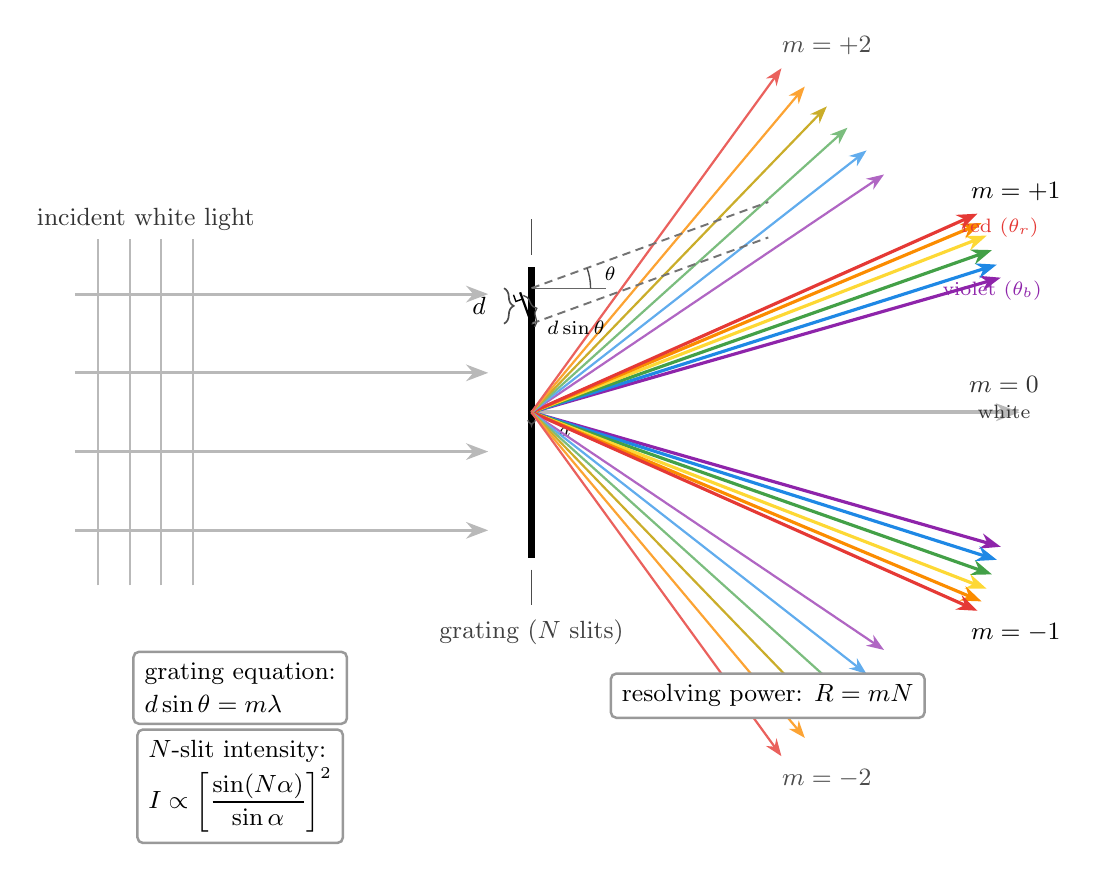
\begin{tikzpicture}[line width=0.9pt, >=Stealth, font=\small]

  % ------- Grating geometry -------
  \def\xG{0}
  \def\slitW{0.09}
  \def\slitH{0.55}
  \def\dd{0.45}
  \def\NSlits{8}
  \pgfmathsetmacro{\ytop}{(\NSlits-1)*\dd/2}

  % ------- Incoming plane wave (white light) on the left -------
  \foreach \x in {-5.5,-5.1,-4.7,-4.3} {
    \draw[gray!55, line width=0.7pt] (\x, -2.2) -- (\x, 2.2);
  }
  \foreach \y in {-1.5, -0.5, 0.5, 1.5} {
    \draw[line width=1.1pt, gray!55, -{Stealth[length=2.8mm]}] (-5.8, \y) -- (-0.55, \y);
  }
  \node[gray!40!black] at (-4.9, 2.45) {incident white light};

  % ------- Grating: row of N small rectangles -------
  \foreach \i in {0,...,7} {
    \pgfmathsetmacro{\y}{\ytop - \i*\dd}
    \fill[black] (\xG-\slitW/2, \y-\slitH/2) rectangle (\xG+\slitW/2, \y+\slitH/2);
  }
  \draw[black!70, line width=0.5pt] (\xG, \ytop+\slitH/2+0.15) -- (\xG, \ytop+\slitH/2+0.6);
  \draw[black!70, line width=0.5pt] (\xG, -\ytop-\slitH/2-0.15) -- (\xG, -\ytop-\slitH/2-0.6);

  % ------- Period d label (on the left of two top slits) -------
  \pgfmathsetmacro{\yA}{\ytop}
  \pgfmathsetmacro{\yB}{\ytop - \dd}
  \draw[decorate, decoration={brace, amplitude=3.5pt}, line width=0.6pt, black!70]
      (\xG-0.35, \yA) -- (\xG-0.35, \yB)
      node[midway, left=3pt, black] {$d$};

  % ------- Slit width a label on one slit -------
  \pgfmathsetmacro{\ySa}{\ytop - 3*\dd}
  \draw[decorate, decoration={brace, amplitude=2pt, mirror}, line width=0.5pt, black!70]
      (\xG-\slitW/2, \ySa-\slitH/2-0.05) -- (\xG+\slitW/2, \ySa-\slitH/2-0.05);
  \node[black, font=\scriptsize] at (\xG+0.42, \ySa-\slitH/2-0.20) {$a$};

  % ------- Grating caption -------
  \node[black!75] at (\xG, -\ytop-\slitH/2-0.95) {grating ($N$ slits)};

  % ------- Outgoing diffracted beams -------
  \coordinate (O) at (\xG, 0);
  \def\Rlen{6.2}

  % m = 0 : white beam straight through
  \draw[line width=1.3pt, gray!55, -{Stealth[length=3mm]}] (O) -- ++(0:\Rlen);
  \node[gray!40!black] at (6.0, 0.35) {$m=0$};
  \node[gray!40!black, font=\scriptsize] at (6.0, 0.0) {white};

  % m = +1 : rainbow fan on upper right (violet inner ~16 to red outer ~24)
  \draw[line width=1.15pt, rviolet, -{Stealth[length=2.6mm]}] (O) -- ++(16.0:\Rlen);
  \draw[line width=1.15pt, rblue,   -{Stealth[length=2.6mm]}] (O) -- ++(17.6:\Rlen);
  \draw[line width=1.15pt, rgreen,  -{Stealth[length=2.6mm]}] (O) -- ++(19.4:\Rlen);
  \draw[line width=1.15pt, ryellow, -{Stealth[length=2.6mm]}] (O) -- ++(21.2:\Rlen);
  \draw[line width=1.15pt, rorange, -{Stealth[length=2.6mm]}] (O) -- ++(22.8:\Rlen);
  \draw[line width=1.15pt, rred,    -{Stealth[length=2.6mm]}] (O) -- ++(24.0:\Rlen);

  % m = -1 : rainbow fan on lower right
  \draw[line width=1.15pt, rviolet, -{Stealth[length=2.6mm]}] (O) -- ++(-16.0:\Rlen);
  \draw[line width=1.15pt, rblue,   -{Stealth[length=2.6mm]}] (O) -- ++(-17.6:\Rlen);
  \draw[line width=1.15pt, rgreen,  -{Stealth[length=2.6mm]}] (O) -- ++(-19.4:\Rlen);
  \draw[line width=1.15pt, ryellow, -{Stealth[length=2.6mm]}] (O) -- ++(-21.2:\Rlen);
  \draw[line width=1.15pt, rorange, -{Stealth[length=2.6mm]}] (O) -- ++(-22.8:\Rlen);
  \draw[line width=1.15pt, rred,    -{Stealth[length=2.6mm]}] (O) -- ++(-24.0:\Rlen);

  % m = +2 : dimmer narrower fan on upper outer side
  \def\Rtwo{5.4}
  \draw[line width=0.8pt, rviolet!70, -{Stealth[length=2.2mm]}] (O) -- ++(34:\Rtwo);
  \draw[line width=0.8pt, rblue!70,   -{Stealth[length=2.2mm]}] (O) -- ++(38:\Rtwo);
  \draw[line width=0.8pt, rgreen!70,  -{Stealth[length=2.2mm]}] (O) -- ++(42:\Rtwo);
  \draw[line width=0.8pt, ryellow!80!black, -{Stealth[length=2.2mm]}] (O) -- ++(46:\Rtwo);
  \draw[line width=0.8pt, rorange!80, -{Stealth[length=2.2mm]}] (O) -- ++(50:\Rtwo);
  \draw[line width=0.8pt, rred!80,    -{Stealth[length=2.2mm]}] (O) -- ++(54:\Rtwo);

  % m = -2 : dimmer narrower fan on lower outer side
  \draw[line width=0.8pt, rviolet!70, -{Stealth[length=2.2mm]}] (O) -- ++(-34:\Rtwo);
  \draw[line width=0.8pt, rblue!70,   -{Stealth[length=2.2mm]}] (O) -- ++(-38:\Rtwo);
  \draw[line width=0.8pt, rgreen!70,  -{Stealth[length=2.2mm]}] (O) -- ++(-42:\Rtwo);
  \draw[line width=0.8pt, ryellow!80!black, -{Stealth[length=2.2mm]}] (O) -- ++(-46:\Rtwo);
  \draw[line width=0.8pt, rorange!80, -{Stealth[length=2.2mm]}] (O) -- ++(-50:\Rtwo);
  \draw[line width=0.8pt, rred!80,    -{Stealth[length=2.2mm]}] (O) -- ++(-54:\Rtwo);

  % Order labels
  \node[black] at (6.15, 2.80) {$m=+1$};
  \node[black] at (6.15,-2.80) {$m=-1$};
  \node[black!70] at (3.75, 4.65) {$m=+2$};
  \node[black!70] at (3.75,-4.65) {$m=-2$};

  % Red / violet labels for m=+1 order
  \node[rred, font=\scriptsize] at (5.95, 2.35) {red ($\theta_r$)};
  \node[rviolet, font=\scriptsize] at (5.85, 1.55) {violet ($\theta_b$)};

  % ------- Path-difference construction between top two slits -------
  \pgfmathsetmacro{\ang}{20}
  \coordinate (S1) at (\xG, \yA);
  \coordinate (S2) at (\xG, \yB);
  \def\Lray{3.2}
  \draw[line width=0.7pt, black!55, densely dashed] (S1) -- ++(\ang:\Lray);
  \draw[line width=0.7pt, black!55, densely dashed] (S2) -- ++(\ang:\Lray);

  % Foot of perpendicular from S2 onto upper ray (through S1 in direction ang)
  \pgfmathsetmacro{\dx}{cos(\ang)}
  \pgfmathsetmacro{\dy}{sin(\ang)}
  \pgfmathsetmacro{\vx}{0}
  \pgfmathsetmacro{\vy}{\yB - \yA}
  \pgfmathsetmacro{\tproj}{\vx*\dx + \vy*\dy}
  \pgfmathsetmacro{\Fx}{\xG + \tproj*\dx}
  \pgfmathsetmacro{\Fy}{\yA + \tproj*\dy}
  \coordinate (F) at (\Fx, \Fy);

  % Perpendicular segment S2 -> F
  \draw[line width=0.8pt, black] (S2) -- (F);
  % Small right-angle marker at F
  \pgfmathsetmacro{\rmk}{0.09}
  \draw[line width=0.5pt, black]
       ($(F) + (\ang+180:\rmk)$)
    -- ($(F) + (\ang+180:\rmk) + (\ang-90:\rmk)$)
    -- ($(F) + (\ang-90:\rmk)$);

  % Brace labeling path difference d sin(theta)
  \draw[decorate, decoration={brace, amplitude=3pt, mirror}, line width=0.5pt, black!70]
       ($(S2)+(0.04,-0.04)$) -- ($(F)+(0.04,-0.04)$)
       node[midway, below right=0pt and 3pt, black, font=\scriptsize]{$d\sin\theta$};

  % theta angle between grating normal and outgoing ray at S1
  \draw[black!60, line width=0.5pt] (S1) -- ++(0:0.95);
  \draw[black!70, line width=0.5pt] ($(S1)+(0.75,0)$) arc[start angle=0, end angle=\ang, radius=0.75];
  \node[black, font=\scriptsize] at ($(S1)+(1.0,0.18)$) {$\theta$};

  % ------- Formula boxes -------
  \node[draw=black!40, rounded corners=2pt, fill=white, inner sep=4pt, align=left, font=\small]
    at (-3.7, -3.5)
    {grating equation:\\[1pt] $d\sin\theta = m\lambda$};

  \node[draw=black!40, rounded corners=2pt, fill=white, inner sep=4pt, align=left, font=\small]
    at (-3.7, -4.75)
    {$N$-slit intensity:\\[1pt] $I \propto \left[\dfrac{\sin(N\alpha)}{\sin\alpha}\right]^{2}$};

  \node[draw=black!40, rounded corners=2pt, fill=white, inner sep=4pt, align=left, font=\small]
    at (3.0, -3.6)
    {resolving power: $R = mN$};

\end{tikzpicture}
\end{document}
